%chktex-file 36
%chktex-file 23
%chktex-file 10
%chktex-file 17
%chktex-file 9
%chktex-file 13
%chktex-file 1
%chktex-file 16
\documentclass[computationalMathematics.tex]{subfiles}

\begin{document}

%%%%%%%%%%%%%%~~~~~~~~~~~~~~~~~~~~~~~~~~~~~~~~~~~~~~~~%%%%%%%%%%%%%%%
\section{11th of October 2018 --- A. Frangioni}
%%%%%%%%%%%%%%~~~~~~~~~~~~~~~~~~~~~~~~~~~~~~~~~~~~~~~~%%%%%%%%%%%%%%%

Last lecture we left with the task of understanding how to check if a function is convex.

As we already stated for convex sets, we can prove that a function is convex deriving from convex functions, though ``convex friendly'' operations.

\begin{myframe}{\bf Note}
There is a softare called~CVX, designed to model convex object. A pretty easy way to check if an object is convex is to try to write it in~CVX.
  If such an operation is possible, then the object is convex. 
\end{myframe}

The following functions are convex:

\begin{enumerate}
  \item $f(x) = w x$: linear functions are both convex and concave;
  \item $f(x) = \frac{1}{2} x Q x + q x$ if convex iff $Q \succeq 0$;
  \item $f(x) = e^{ax}$ for any $a \in \R$ and $x \in \R$
  \item $f(x) = -\log(x)$ for $x > 0$
  \item $f(x) = x^a$ for $a \geq 1$ or $a \leq 0$ on $x \geq 0$;
  \item $f(x) = \norm{x}_p$ for $p \geq 1$;
  \item $f(x) = \max \{x_1, \ldots, x_n\}$;
  \item for any convex set $C$, its indicator function
        \[
         \mbox{\i}_C(x) =
         \left\{\begin{array}{cc} 0 & \mbox{if } x \in C \\
                            +\infty & \mbox{if } x \notin C
                \end{array}\right.
         \mbox{(l.s.c.} \iff C \mbox{ closed)}
        \]
  \item $A \in \R^{n \times n}$ symmetric, eigenvalues customarily ordered $\lambda_1 \geq \lambda_2 \geq \ldots \lambda_n$: $f_m(A) = \sum\limits_{i = 1}^m \lambda_i$ (sum of $m$ largest eigenvalues)
\end{enumerate}

\begin{proposition}
The following operations preserve convexity:

\begin{enumerate}
 \item $f$, $g$ convex, $\alpha$, $\beta \in \R_+ \Longrightarrow \alpha f + \beta g$ convex (non-negative combination);
 \item ${\{f_i\}}_{i \in I}$ (infinitely many) convex functions $\Longrightarrow f(x) = \sup_{i \in I} f_i(x)$ convex, see \Cref{subfloat:11ott_1};
 \item Pre-composition with linear function is convex, formally $f$ convex $\Longrightarrow f(Ax + b)$ convex;
 \item Post-composition with increasing convex function is convex. Formally, $f : \R^n \to \R$ convex, $g : \R \to \R$ convex increasing $\Longrightarrow$ $g \circ f = g(f(x))$ is convex;
 \item $f_1$, $f_2$ convex $\Longrightarrow f(x) = \inf \{ \, f_1(x_1) + f_2(x_2)~:~x_1 + x_2 = x\}$ convex (infimal convolution);
 \item $g$ convex $\Longrightarrow f(x) = \inf \{g(y)~:~Ay = x\}$ convex (image under a linear mapping, aka value function of convex constrained problem);
 \item $g(x,y) : \R^{n + m} \to \R$ convex $\Longrightarrow f(x) = \inf \{g(x,y)~:~y \in \R^m\}$ convex (partial minimization);
 \item $f(x)$ convex $\Longrightarrow \tilde{f}(x,u) = u f(x / u)$ when $u > 0$, $\tilde{f}(x,u) = \infty$ otherwise, convex (perspective or dilation function of $f$), see \Cref{subfloat:11ott_2}.
\end{enumerate}
\end{proposition}

\begin{figure}[h]
  \centering
  \subfloat[][Suprema --- second property]{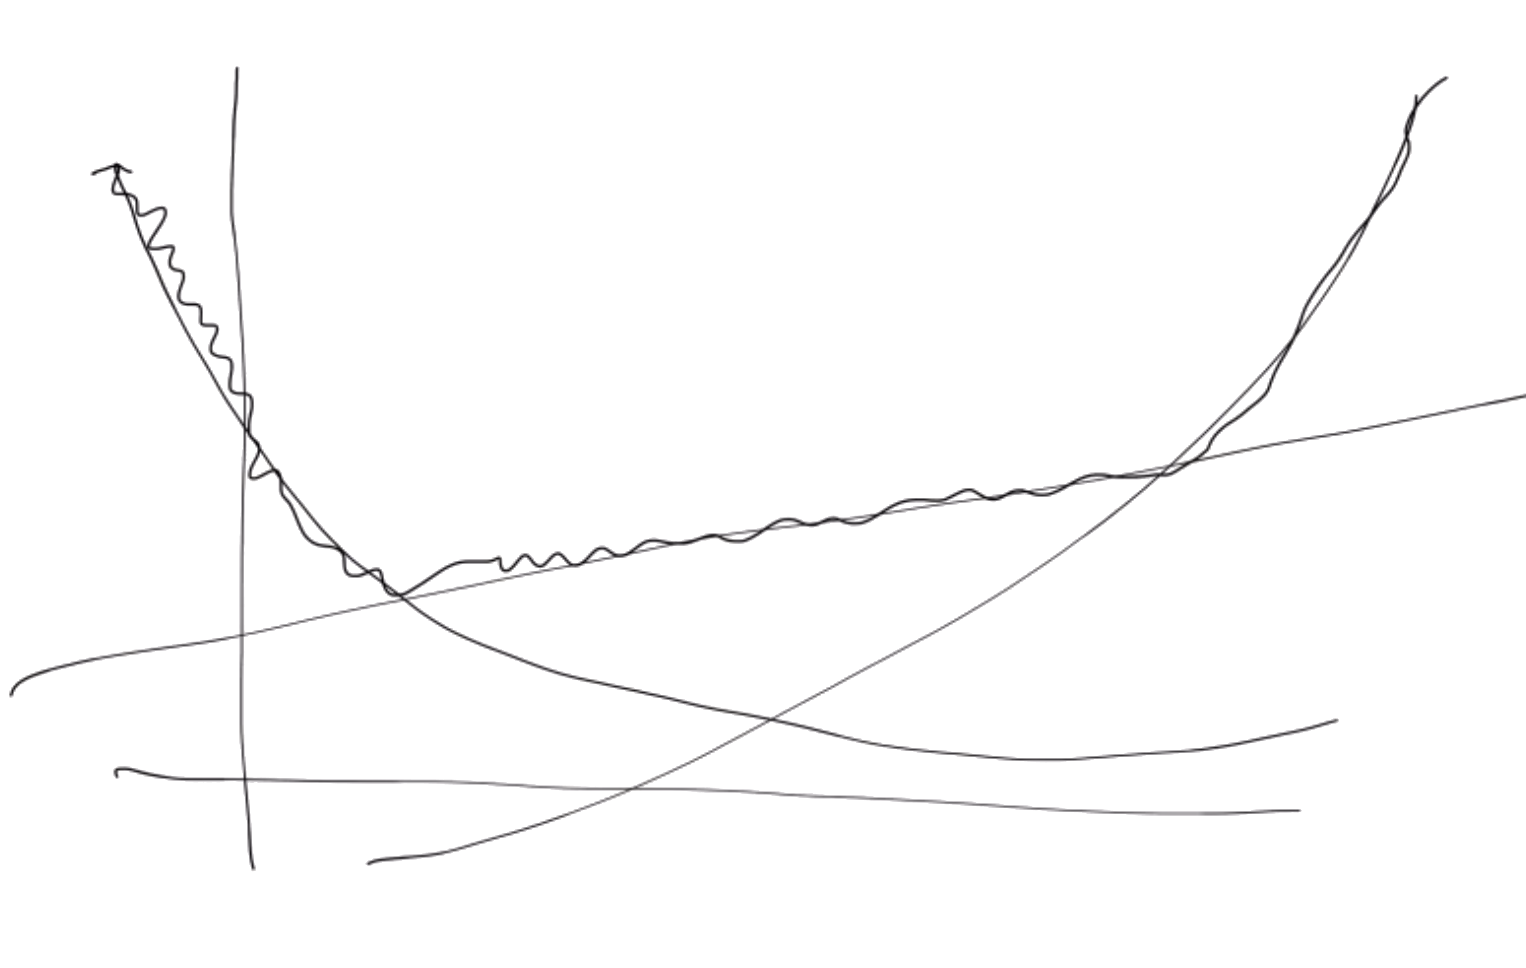
\includegraphics[width=0.35\textwidth]{pics/11ott/sup.png}\label{subfloat:11ott_1}}
  \hspace{0.5cm}
  \subfloat[][Perspective --- eightth property]{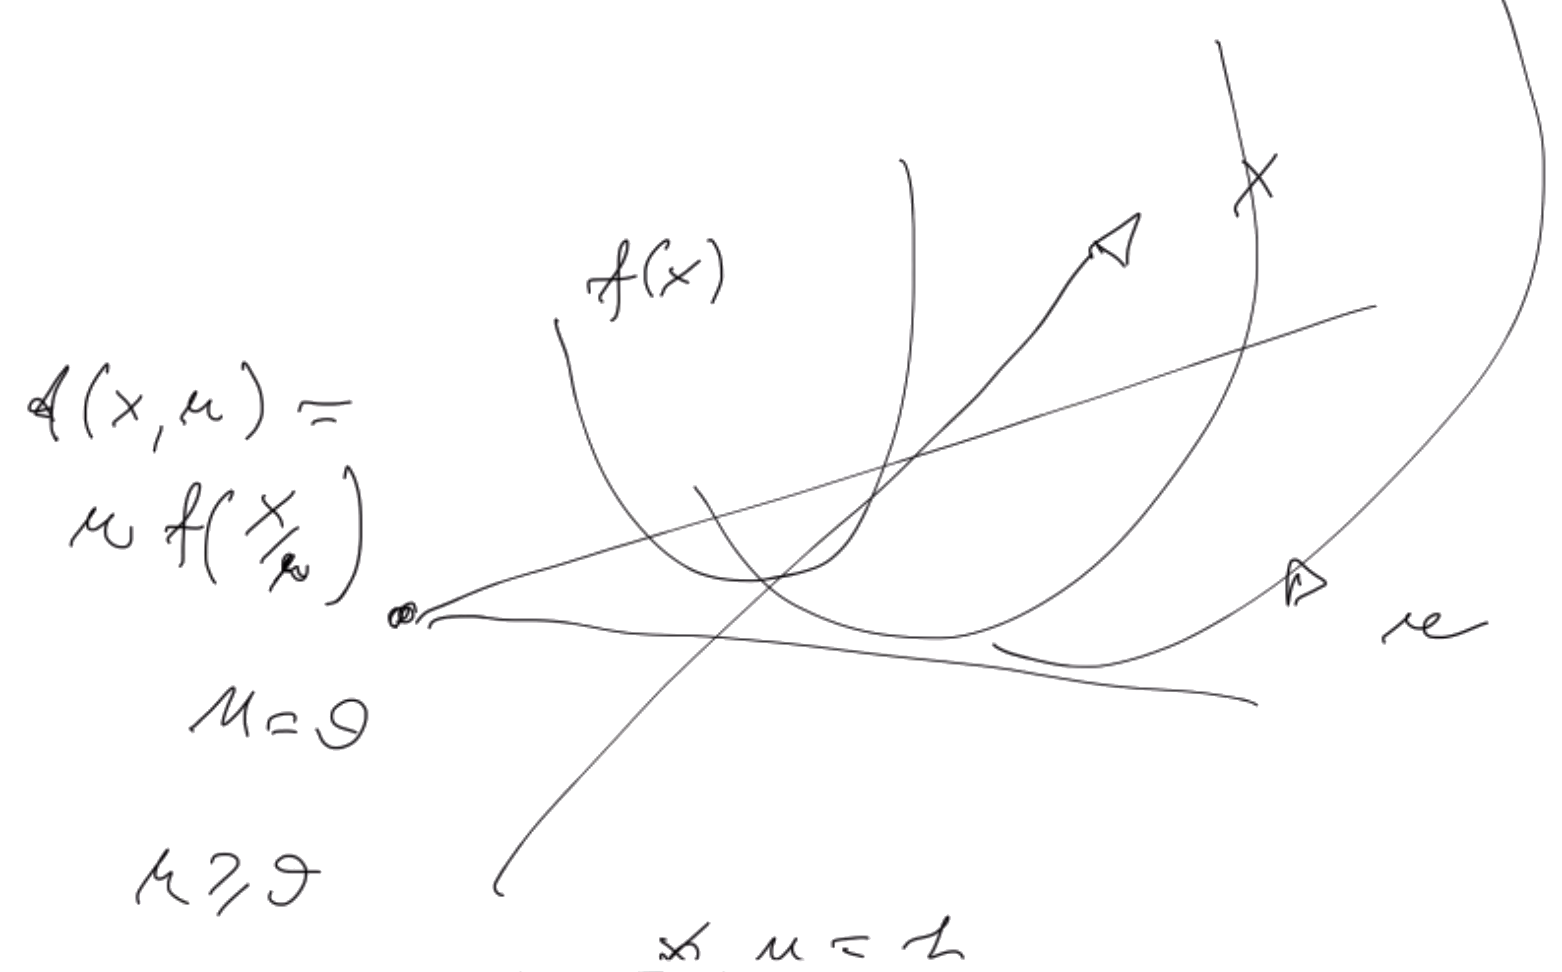
\includegraphics[width=0.35\textwidth]{pics/11ott/perspective.png}\label{subfloat:11ott_2}}\\
  \caption{Graphic hints.}\label{fig:11ott_1}
\end{figure}

\begin{proposition}
  Let $f: \R^n \to \R \cup {\infty}$ a convex function. If $\exists \bar{x} \in dom(f)$ such that $f(\bar{x}) = - \infty$, then $f \equiv - \infty$. 
\end{proposition}

From now on we will solve the issue of functions with non convex domain, sayting that in those points where the function is not defined, we value it $+ \infty$.

\begin{proposition}\label{prop:11ott_1}
  Let $f: \R^n \to \R$ be a convex function. Then $f$ is Lipschitz continuous $\forall$ bounded convex set $S \subseteq \text{int(dom(}f$)) but on $\partial dom(f)$ (the border of the domain) anything can happen.

  Moreover, a function $f$, which is continuous but not Lipschitz continuous is not convex.
\end{proposition}

A couple of examples of \Cref{prop:11ott_1} can be found in \Cref{fig:11ott_2}.

\begin{figure}[h]
  \centering
  \subfloat[][Take a compact set in the interior of the domain (far from the boundaries) there the function is Lipschitz continuous.]{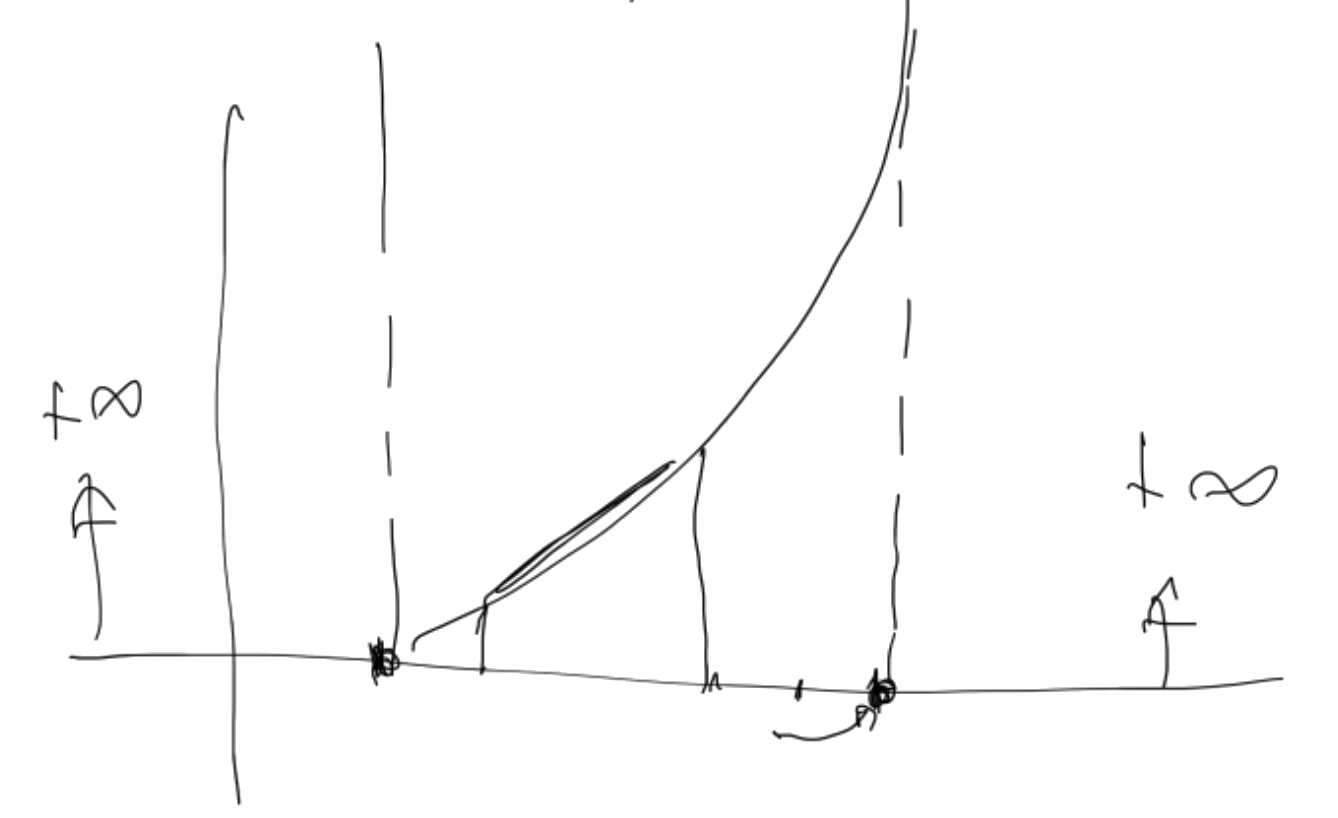
\includegraphics[width=0.35\textwidth]{pics/11ott/lip1.png}\label{subfloat:11ott_3}}
  \hspace{0.5cm}
  \subfloat[][If a function is not Lipschitz on a compact subset it is not convex.]{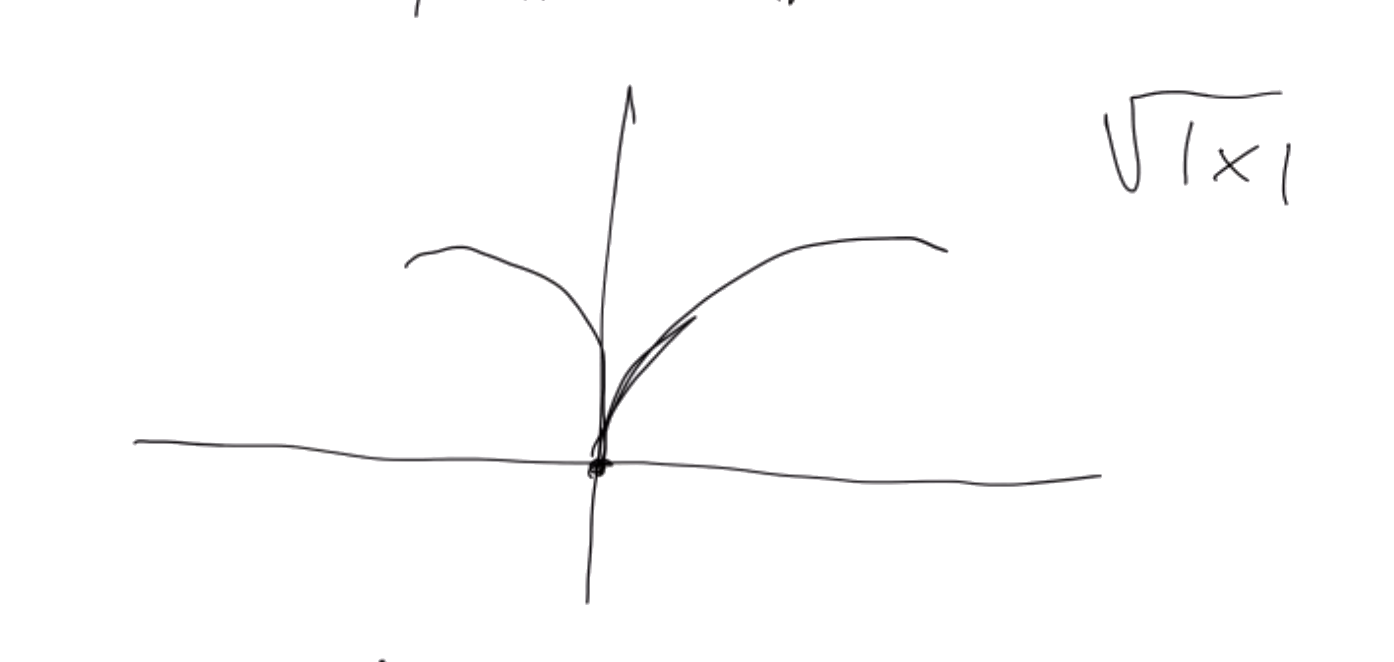
\includegraphics[width=0.45\textwidth]{pics/11ott/lip2.png}\label{subfloat:11ott_4}}\\
  \caption{}\label{fig:11ott_2}
\end{figure}

\begin{proposition}
Let convex $f: \R^n \to \R$. Then it is Lipschitz continuous on any bounded set and continuous everywhere.
\end{proposition}

It happens often that the set of points in which a function is non differentiable have measure $0$.

\begin{theorem}[Convexity characterization]
Let $f \in C^1$. It is convex on $C$ convex iff
\[
  f(y) \geq f(x) + \nabla f(x) ( \, y - x \, ) \forall \, x,y \in C
\]

In other words, given a point $x$, we compute the derivative and the value fo the function is above the derivative in that point.
\end{theorem}

\begin{proof}
  \begin{description}
    \item[$\Rightarrow)$]
      $\alpha (f(y) - f(x)) \geq f( \alpha (y - x) + x) - f(x)$, send $\alpha \to 0$
    \item[$\Leftarrow)$]TODO
  \end{description}
\end{proof}

\begin{theorem}
Let $f \in C^1$ convex. $x$ is a stationary point iff $x$ is a global minimum.
\end{theorem}

\begin{proposition}
  Let $f$ be twice differentiable (aka has Hessian). $f$ is convex iff the Hessian is positive semidefinite.

  Formally, let $f \in C^2$. $f$ is convex on the open set $S$ iff $\nabla^2 f(x) \succeq 0~\forall x \in S$.
\end{proposition}

This proposition gives us an algorithm to check if a function is convex or not: we only need to compute the eigenvalues of the Hessian and check if they are positive.

There are some functions which do not have differentiability property.

A way to work with functions which are not defined on all $\R$ is to solve the following problem:

\[
  (P) \equiv \inf \{f_X(x) = f(x) + \i_X(x)~:~x \in \R^n\}
\]

thanks to

\begin{theorem}[Essential objective]
$x_*$ optimal for $(P)$ $\iff$ $x_*$ local minimum of $f_X$.
\end{theorem}

\subsubsection{Subgradients and subdifferentials}

\begin{definition}[Subgradient]
  For each $s \in \R$ we term \textbf{s-subgradient} of $f$ at $x$ as
  
\[
  f(y) \geq f(x) + s (y - x) \qquad \forall \, y \in \R^n
\]
\end{definition}

Let us assume that the minimum of the non differentiable function resides in one of its kiky points, then for $s=0$ we have a subgradient which is flat and this is a sufficient condition for minimality, for a pictorial example see \Cref{fig:11ott_3}.

\addpic{0.5}{pics/11ott/convexnondiff09.pdf}{Pictorial example of subgradients of a non diffrentaible function.}{fig:11ott_3}

The issue here is that it is unfeasible to check if the subgradient with $s=0$ is a subgradient for $f$.

\begin{definition}[Subdifferential]
  We term \textbf{subdifferential} the set of all possible subgradients.

  Formally,
  \[
    \partial f(x) := \{s \in \R^n~:~s \text{ is a subgradient at } x\} 
  \]
\end{definition}


\begin{theorem}
$x$ global minimum $\iff 0 \in \partial f(x)$.
\end{theorem}

Notice that in general, when we are not in proximity of a border (where $f$ is unbounded above) we get that the subdifferential is a compact interval.

Formally,$\partial f(x)$ closed and convex, compact $\forall \, x \in int \, dom(f)$.

Moreover, we can prove the following

\begin{proposition}
$\partial f(x) = \{\nabla f(x)\} \iff f$ differentiable at $x$.
\end{proposition}

An attentive reader may have noticed that in the case of non differentiable functions it is not possible to derive the directional derivative from the gradient ($\frac{\partial f}{\partial d}(x) = \ps{\nabla f(x)}{d}$), but we can prove the following

\begin{proposition}
$\frac{\partial f}{\partial d}(x) = \sup \{\ps{s}{d}~:~s \in \partial f(x)\} \Longrightarrow$ $d$ is a descent direction  $\iff \ps{s}{d} < 0~\forall~s \in \partial f(x)$.
\end{proposition}

As in the differentiable case, we are interested in moving in the steepest descent direction, formally $s_* = - \mbox{argmin} \{\norm{s}~:~s \in \partial f(x)\}$.

\begin{example}
Le us assume we are in $x$ and we want to move towards $x^*$ knowing only the subdifferentials.
$(-)\partial f(x)$ is convex and compact and All $(-)g \in \partial f(x)$ ``point towards $x_*$'': $\ps{g}{x - x_*} < 0$.

Not all of them are descent directions, but the (opposite to the) minimum-norm one is a descent direction.

  \addpic{0.3}{pics/11ott/nondiffrn09.pdf}{There are many different subgradients in $x$. We pick the one with minimum norm among the ones which have a negative scalar product with $x - x^*$.}{fig:11ott_3}
\end{example}

Notice that in $\R^2$ if we take a function and compute the subdifferential, we can scale both the function and the subdifferential by any positive constant (negative contants would lead to concave functions). Formally,

\begin{proposition}
Let $f,g: \R^n \to \R$ and take $\alpha, \beta \in \R_+$, then $\partial [\alpha f + \beta g](x) = \alpha \partial f(x) + \beta \partial g(x)$.
\end{proposition}

\begin{proposition}[Chain rule]
  \begin{itemize}
    \item Let $f: \R^n \to \R$ and let $A \in M(n, \R)$ and $b \in R^n$ then $\partial [f(Ax + b)] = A^T [\partial f](Ax + b) $;
    \item $g:\R \to \R$ increasing, then $\partial [g(f(x))] = [\partial g](f(x)) [\partial f](x)$.
  \end{itemize}
\end{proposition}

\begin{definition}[$\eps$-subgradient]
  Let $f: \R^n \to \R$. $s$ is $\varepsilon$\textbf{-subgradient} at $x$ if 
\[
  f(y) \geq f(x) + s (y - x) - \varepsilon~ \forall y \in \R^n
\]
support hyperplane passing $\varepsilon$ below $epi(f)$
\end{definition}

\begin{proposition}
Given a point $x$, the value of the finction in $x$ cannot be further from $\eps$ the minimum value fo the function.
  Formally, $0 \in \partial_\varepsilon f(x) \iff x$ is $\varepsilon$-optimal. 
\end{proposition}

We are now allowed to compute $s_* = \mbox{argmin} \{\norm{s}~:~ s \in \partial_\varepsilon f(x)\}$.

If $s_* = 0$ then $x$ is $\eps$ optimal. Otherwise, $\exists \alpha > 0$ s.t.~$f(x - \alpha s_*) \leq f(x) - \varepsilon$ ($- s_*$ is of $\varepsilon$-descent).

The $\eps$-subgradient is very powerful, but the issue is that is even more expensive to compute than the subgradient.

\end{document}
